\documentclass[12pt, a4paper]{article}
\usepackage[T1]{fontenc}
\usepackage[utf8]{inputenc}
\usepackage{mathpazo}
\usepackage{microtype}
\usepackage{geometry}
\geometry{margin=1.2in}
\usepackage{amsmath, amssymb, amsthm}
\usepackage{booktabs}
\usepackage{array}
\usepackage{xcolor}
\usepackage{tikz}
\usepackage{pgfplots}
\pgfplotsset{compat=1.18}
\usepackage{hyperref}
\usepackage{setspace}
\usepackage{enumitem}
\usepackage{float}
\usepackage{caption}

\onehalfspacing

\definecolor{fogblue}{RGB}{100,130,170}
\definecolor{obscuregray}{RGB}{140,140,140}
\definecolor{alarmred}{RGB}{180,40,40}

\newtheorem{definition}{Definition}
\newtheorem{theorem}{Theorem}
\newtheorem{proposition}{Proposition}
\newtheorem{observation}{Observation}
\newtheorem{remark}{Remark}

% Simple callout box using quote environment + rule
\newenvironment{claritybox}
  {\begin{quote}\small\color{fogblue}\rule{\linewidth}{0.6pt}\par\smallskip}
  {\par\smallskip\rule{\linewidth}{0.4pt}\end{quote}}

\newenvironment{metricbox}
  {\begin{quote}\small\color{obscuregray}\rule{\linewidth}{0.4pt}\par\smallskip}
  {\par\smallskip\rule{\linewidth}{0.4pt}\end{quote}}

\newenvironment{warnbox}
  {\begin{quote}\small\color{alarmred}\rule{\linewidth}{0.6pt}\par\smallskip}
  {\par\smallskip\rule{\linewidth}{0.4pt}\end{quote}}

\hypersetup{colorlinks=true, linkcolor=fogblue, urlcolor=fogblue, citecolor=fogblue}

\title{%
  \textbf{The Unreadability of Dynamic Readability:}\\
  \large An Explicit Specification of a Conceptualization\\[0.5em]
  \normalsize\textit{With Progressive Methodological Refinement and\\
  Increasingly Rigorous Framework Instantiation}
}
\author{%
  Flyxion\\
  \small Independent Researcher\\
  \small \texttt{github.com/standardgalactic}
}
\date{\small Working Paper --- Circulated for Comment}

\begin{document}

\maketitle
\thispagestyle{empty}

\begin{abstract}
This paper investigates the phenomenon of dynamic unreadability as instantiated within and through academic discourse, attending particularly to the mechanisms by which communicative opacity is generated, sustained, and mistaken for intellectual depth. The argument proceeds from a simple premise --- that clarity is not simplification, but navigability --- and demonstrates this thesis by example, the example in question being the present paper itself.

We introduce several analytical tools: the Semantic Density Ratio (SDR), the Referential Fog Index (RFI), the Recursive Qualification Depth (RQD), and the Average Noun Stack Length (ANSL). We further develop a distinction between World-Topological Coupling (WTC) and Citation-Topological Closure (CTC) as diagnostic indices of disciplinary epistemic health. We compare contemporary academic obscurantism unfavorably with the visual epistemology of Athanasius Kircher, whose diagrams demonstrate that density and navigability are not, in principle, opposed.

The paper's formal properties will be found to undergo a gradual transformation across its sections. Readers are encouraged to notice this.
\end{abstract}

\newpage
\tableofcontents
\newpage

%======================================================
\section{Introduction: A Simple Problem, Simply Stated}
%======================================================

\begin{claritybox}
\textbf{Plain statement of the thesis:} Academic writing is often difficult to read not because the ideas are complex, but because the writing is optimized for the wrong things. This paper examines that problem --- and, in doing so, demonstrates it.
\end{claritybox}

Have you ever begun the opening paragraph of a peer-reviewed paper and discovered, halfway through the page, that your cognitive faculties have staged a silent revolt? You were reading words. The words were English. The sentences were grammatical. And yet something had gone wrong somewhere, in the way that a perfectly legal sequence of turns can leave you facing a wall in a parking garage with no obvious exit.

This is not a failure of intelligence. It is a failure of architecture.

Academic writing, at its worst, is not merely complex. It is labyrinthine without being interesting, dense without being informative, authoritative without being grounded. It mistakes the appearance of rigor for rigor itself. It uses obscurity the way a squid uses ink: not to hide something dangerous, but simply because it seems to help with social survival in murky environments.

The question this paper asks is simple: why does this happen, and what would it mean to do otherwise?

\subsection{What Clarity Is Not}

A common response to obscure academic writing is to call for simplicity. Write shorter sentences. Avoid jargon. Explain your terms. Use examples. This advice is not wrong, exactly, but it misses the deeper issue.

Some of the clearest writing is also the most technically demanding. A well-constructed mathematical proof can be followed by a careful reader who has never encountered the specific problem before, not because it avoids complexity, but because it scaffolds that complexity carefully. Each step is visible. Each inference is explicit. The reader can orient themselves within the argument at every moment.

Conversely, some of the most impenetrable writing consists of simple words arranged into conceptual fog. The sentences are short. The vocabulary is accessible. And yet nothing connects. There is no ground beneath the prose, no load-bearing architecture, only an accumulation of gestures toward ideas that never quite arrive.

\begin{claritybox}
\textbf{Working definition:} \textit{Clarity is not simplicity. Clarity is navigability: the property of a symbolic structure that allows a reader to maintain orientation within it under bounded cognitive conditions.}
\end{claritybox}

\subsection{The Paper Ahead}

The paper is organized as follows. Section~2 introduces a brief taxonomy of academic difficulty, distinguishing modes of density that serve understanding from modes that merely perform it. Section~3 develops our core analytical metrics. Section~4 examines the phenomenon of citation-topological closure. Section~5 considers Kircher as an unexpected model of dense-but-navigable information design. Section~6 introduces the Swedenborgian Coherence Response as a model of reader overload under high symbolic saturation. Section~7 provides the paper's central formal apparatus. Section~8 applies that apparatus to the paper itself. Section~9 concludes.

Readers who find the paper increasingly difficult to follow as it progresses are responding correctly.


%======================================================
\section{A Taxonomy of Difficulty}
%======================================================

Not all difficult writing is the same. Before we can diagnose academic obscurantism, we need to distinguish it from the several legitimate forms of textual density it superficially resembles.

\subsection{Productive Density}

Some writing is difficult because the underlying structure is genuinely complex. Consider tensor calculus. The notation is compact, the abstraction is high, and a reader without training will find it opaque. But this opacity is not a rhetorical failure. It is the necessary consequence of compressing an enormous amount of precisely specified relational structure into a small symbolic space. The difficulty is proportional to the content.

A reader who acquires the necessary background infrastructure will find that the notation becomes transparent. The difficulty was not in the writing; it was in the prerequisite knowledge, which the notation presupposes rather than reconstructs. This is productive density: symbolic compression that preserves and rewards interpretive effort.

\subsection{Compressive Shorthand}

Expert communities necessarily develop shorthand. A phrase like ``variational free-energy minimization under Markov blanket formalism'' is opaque to an outsider, but within active predictive-processing research communities it efficiently references a large, well-specified conceptual architecture. This is not obscurantism. It is specialization. The problem arises not when expert shorthand exists, but when it migrates out of context without reconstruction.

\subsection{Ritualized Obscurity}

Here the pathology begins. Ritualized obscurity occurs when complexity functions socially rather than informationally. The language is difficult not because the ideas require difficulty, but because opacity itself has become institutionally valuable: it signals disciplinary membership, theoretical sophistication, or the kind of serious-minded engagement that attracts grant funding and tenure consideration.

The tell-tale sign is that paraphrase is possible without loss. If you can translate a passage into plain language and nothing of substance is lost, then the complexity was not serving the ideas; it was serving the author's institutional positioning.

\subsection{Adversarial Opacity}

In its terminal form, obscurity actively resists comprehension. This may result from recursive qualification, in which every claim is so thoroughly hedged that it commits to nothing; from unstable terminology, in which key terms shift meaning across sections without announcement; from excessive noun-stacking, in which pre-nominal modifier chains grow too heavy to parse; or from what we might call semantic vapor --- the production of syntactically correct sentences that fail to resolve into any coherent proposition on inspection.

\begin{claritybox}
\textbf{Heuristic:} Ask, after reading a passage: \textit{what would it mean for this to be wrong?} If the question cannot be answered, the passage may be producing semantic vapor regardless of its surface complexity.
\end{claritybox}


%======================================================
\section{Preliminary Metrics: A First Approximation}
%======================================================

With the taxonomy in place, we can begin to formalize. The following metrics are introduced with a degree of seriousness that we leave intentionally ambiguous.

\subsection{Semantic Density Ratio (SDR)}

\begin{definition}[Semantic Density Ratio]
For a text $T$, the Semantic Density Ratio is:
\[
\mathrm{SDR}(T) = \frac{I(T)}{L(T)}
\]
where $I(T)$ denotes the informational content of $T$ and $L(T)$ denotes its lexical opacity.
\end{definition}

We acknowledge, with a candor unusual in technical writing, that neither $I(T)$ nor $L(T)$ admits of straightforward measurement. The important thing is the ratio: a text can be lexically opaque and informationally rich (high SDR), or lexically opaque and informationally sparse (low SDR). The latter case is the pathological one.

\begin{table}[H]
\centering
\caption{Illustrative SDR scores for representative text types}
\begin{tabular}{lc}
\toprule
\textbf{Text type} & \textbf{SDR (approximate)} \\
\midrule
Advanced mathematical proof & High \\
Well-written science journalism & High \\
Technical specification document & Moderate--High \\
Peer-reviewed humanities paper & Variable \\
Grant proposal (committee-authored) & Low \\
Conference keynote (plenary) & Very Low \\
\bottomrule
\end{tabular}
\end{table}

\subsection{Referential Fog Index (RFI)}

\begin{definition}[Referential Fog Index]
The Referential Fog Index $\mathrm{RFI}(T)$ measures the proportion of the interpretive load borne by implicit reference to external theoretical frameworks, relative to what is reconstructed within $T$ itself.
\end{definition}

A text with high RFI cannot be understood without extensive background in a specific theoretical tradition, not because the ideas themselves are inaccessible, but because the author has chosen not to reconstruct the scaffolding. Consider: ``Within a post-Deleuzian deterritorialization framework informed by post-Lacanian affect topology, the subject is understood as\ldots'' The difficulty here is not conceptual; it is genealogical.

\subsection{Recursive Qualification Depth (RQD)}

\begin{definition}[Recursive Qualification Depth]
For a proposition $P$, the Recursive Qualification Depth $\mathrm{RQD}(P)$ is the number of nested hedging operations applied to $P$ before its surface-level assertion.
\end{definition}

For illustration: the proposition \textit{``Obscure writing is sometimes intentional''} has $\mathrm{RQD} = 0$. The proposition \textit{``It might reasonably be suggested that, under certain institutional conditions, some forms of what could provisionally be characterized as deliberate opacity may be, in a non-trivial sense, potentially intentional''} has $\mathrm{RQD} = 6$.

\subsection{Average Noun Stack Length (ANSL)}

\begin{definition}[Average Noun Stack Length]
$\mathrm{ANSL}(T)$ is the mean length of pre-nominal modifier chains across all noun phrases in a text $T$.
\end{definition}

For readable academic prose, ANSL typically falls between 1.2 and 1.8. Above 2.5, readers begin to experience noun-stack overflow: the working memory required to parse the phrase exceeds the capacity available while tracking the sentence's broader syntactic structure. The noun phrase ``post-structuralistic ontological paradigm destabilization framework instantiation'' has a pre-nominal stack depth of 4. It does not reward the effort.


%======================================================
\section{Citation-Topological Closure: A Theoretical Digression Which Will Prove Germane}
%======================================================

Having established the basic metric apparatus (which will be further extended in due course, with appropriate refinements to notation and scope), we now turn to what is perhaps the deepest structural problem in academic discourse: the progressive decoupling of discourse from the world it purports to describe.

\subsection{World-Topological Coupling}

A healthy intellectual discipline maintains what we shall term high World-Topological Coupling (WTC): its propositions remain connected, through a traceable chain of inference and evidence, to phenomena in the world. Theories are tested. Predictions are made. Anomalies generate revisions.

\begin{definition}[World-Topological Coupling]
The World-Topological Coupling $\mathrm{WTC}(\mathcal{D})$ of a discourse $\mathcal{D}$ is a measure of the density of evidential and inferential paths connecting propositions in $\mathcal{D}$ to non-discursive phenomena.
\end{definition}

High WTC discourses are harder to maintain because the world pushes back. Low WTC discourses are institutionally easier: nothing external can falsify them, because nothing external was ever incorporated as a constraint.

\subsection{Citation-Topological Closure}

\begin{definition}[Citation-Topological Closure]
A discourse $\mathcal{D}$ exhibits Citation-Topological Closure (CTC) to degree $\alpha$ when a proportion $\alpha$ of its propositions derive authority primarily from their position within citation networks, rather than from direct connection to empirical or phenomenological substrates.
\end{definition}

In a citation-topologically closed discourse, papers cite papers which cite papers. Frameworks reference frameworks. Terminology stabilizes not by achieving precision but by circulating long enough to acquire the patina of established usage. The internal coherence of the network increases while its world-contact silently decays.

\begin{observation}
Citation-topological closure is self-reinforcing: in a closed discourse, citations to world-grounded work appear methodologically naive (``insufficiently theoretical''), while citations to highly theoretical work appear sophisticated regardless of their empirical traction. The institutional reward gradient thus accelerates closure.
\end{observation}

Let us define the World-Anchor Density $\rho_W(\mathcal{D})$ of a discourse as the number of evidential anchors per unit of propositional content. As $\rho_W \to 0$, the discourse becomes progressively self-indexing: each proposition is warranted by reference to other propositions, which are warranted by reference to yet others, forming a structure that is internally consistent but externally unanchored.

\begin{proposition}
A discourse approaching citation-topological closure will exhibit increasing internal coherence metrics (citation connectivity, terminological consistency, framework stability) simultaneously with decreasing world-contact. These metrics are therefore not reliable indicators of epistemic health in isolation.
\end{proposition}

This has an important practical corollary. Disciplines that evaluate their own epistemic progress using citation metrics are measuring the wrong thing. A rising citation-topological closure coefficient may look, from the inside, like increasing theoretical sophistication. From the outside, it looks like a particularly well-organized hall of mirrors.


%======================================================
\section{The Kircherian Interlude: Density Without Fog}
%======================================================

Before we proceed to the more formally elaborate sections of this paper (in which the preceding framework will be extended, refined, and in certain respects retroactively reconsidered), it is worth pausing to examine an apparent counterexample to the thesis that academic density is necessarily hostile to navigation.

Athanasius Kircher (1602--1680), Jesuit polymath, produced some of the most informationally overloaded documents in the history of European scholarship. His \textit{Mundus Subterraneus}, his \textit{Oedipus Aegyptiacus}: these works pile symbolic systems atop each other, layer cosmological speculation onto linguistic analysis onto natural philosophy onto theological allegory, in a way that ought to be entirely unnavigable.

And yet --- they are not, quite.

\subsection{Architectural vs.\ Ornamental Density}

The reason Kircher's diagrams remain legible despite their overload is that they are organized architecturally rather than linearly. Information is spatially deployed. The reader's eye finds purchase in the structure of the page before it attempts to parse individual elements. Relationships are made visible geometrically: concentricity, hierarchy, radial symmetry, inclusion and exclusion. The cognitive load is real, but it is distributed across a navigable space rather than compressed into an impenetrable sequence.

Modern academic prose, by contrast, tends toward ornamental density: lexical complication that has no geometric organization, that must be processed linearly word-by-word without structural landmarks.

\begin{claritybox}
\textbf{The Kircherian distinction:} Dense-but-navigable complexity is architecturally organized. It distributes cognitive load across a legible structure. Dense-but-unnavigable complexity lacks this architecture; it produces lexical mass without mnemonic geometry.
\end{claritybox}

\subsection{What We Inherited, and What We Lost}

Kircher was wrong about almost everything. His hieroglyphic decipherments were fantasies. His underground fire system was incorrect. And yet the failure was, in a sense, navigable: it was possible to identify what he had claimed, to test it, to show that it was incorrect. Much contemporary theoretical obscurantism is not even navigably wrong. It cannot be shown to be false because it cannot be shown to claim anything definite.

We inherited the density. We lost the cathedral.


%======================================================
\section{Swedenborgian Overload States and Visionary Rendering Failure}
%======================================================

An important precursor to contemporary informational overload may be observed in the visionary experiences of Emanuel Swedenborg (1688--1772). Swedenborg's cosmological visions --- vast architectural heavens, recursive symbolic correspondences, multilayered moral geographies, angelic communication systems, and dynamically interconnected spiritual ecologies --- are often treated either as mystical revelations or psychiatric anomalies. Both interpretations may obscure an important structural feature of the experiences themselves: they resemble the phenomenology of a symbolic rendering system operating beyond stable cognitive bandwidth.

To state the matter provocatively but not entirely inaccurately: Swedenborg's visions behaved less like linear propositions and more like GPU overload hallucinations.

This comparison should not be understood dismissively. Modern graphical processing systems exhibit a revealing failure mode under excessive load. As rendering demands exceed available resources, the system begins fragmenting geometry, overextending pattern interpolation, recursively duplicating textures, hallucinating continuity between partially rendered objects, and generating unstable but locally coherent visual spaces that have no stable relationship to the scene description from which they were computed.

Something structurally similar appears in Swedenborgian visionary architecture. Symbolic density exceeds the stable navigational capacity of ordinary cognition. The mind compensates through recursive synthesis, generating increasingly elaborate correspondence structures in an attempt to maintain coherence across overwhelming semantic throughput.

The resulting visions are therefore neither arbitrary fantasies nor stable revelations. They are dynamic compensatory renderings produced under conditions of conceptual oversaturation.

\subsection{Swedenborg as Diagnostic Instrument}

This interpretation becomes especially relevant when considering highly recursive academic discourse. At sufficient levels of symbolic density, readers begin exhibiting what we shall term Swedenborgian compensation effects: constructing implied coherence where none is explicitly present; inferring hidden structure from typographic salience; assigning significance to recursive terminology; and hallucinating explanatory continuity across disconnected conceptual regions.

The modern academic paper, especially in its most citation-topological forms, increasingly resembles a low-frame-rate cosmological rendering engine attempting to maintain the illusion of navigable semantic continuity while operating beyond human interpretive bandwidth.

This may explain the peculiar phenomenology of certain theoretical texts. Readers often report that they \textit{feel} profound coherence before they can identify any recoverable proposition. The paper generates an atmospheric conviction of significance independent of explicit conceptual traversal. The effect is strongest in papers with high $J_s^2$ and low $\rho_W$: dense jargon, weak world-contact, maximum atmospheric pressure.

\begin{definition}[Swedenborgian Coherence Response]
\label{def:scr}
The Swedenborgian Coherence Response is:
\[
\mathrm{SCR}(T) = \frac{A_s(T)}{R_p(T)}
\]
where $A_s(T)$ denotes ambient symbolic density and $R_p(T)$ denotes the count of recoverable propositions.
\end{definition}

At high $\mathrm{SCR}$ values, the reader experiences intense interpretive gravity despite declining semantic recoverability. This is not a failure of reading; it is a rational response to an environment that has been optimized --- whether intentionally or through institutional drift --- to produce the sensation of significance as a substitute for its substance.

\subsection{The Rendering Failure Generalized}

Importantly, this phenomenon is not unique to mysticism or theory. Financial systems, bureaucratic institutions, large software stacks, and contemporary AI discourse all increasingly exhibit Swedenborgian rendering characteristics: locally coherent symbolic overproduction under conditions of global interpretive overload. The problem is therefore not hallucination in the ordinary sense. The problem is that sufficiently overloaded symbolic systems begin generating atmospheric coherence fields that exceed the capacity of any participant to fully traverse them.

The Kircher comparison becomes even more precise here. Kircher's overload was architecturally organized; the reader could enter it, navigate it, and exit with recoverable propositions, however wrong those propositions might be. Swedenborg's overload --- and the discourse overload of late citation-topological closure --- is not organized for navigation. It is organized for immersion. The reader is meant to \textit{feel} understood rather than to \textit{become} informed.

This distinction maps cleanly onto the WTC/CTC framework: Kircherian density maintains world-topological coupling while maximizing symbolic load. Swedenborgian density achieves citation-topological closure at the level of the individual cognitive event, generating internal coherence at the expense of external recoverability.

For readability reasons, several intermediate stages of the derivation have been omitted.\footnote{The reader familiar with Section~3 will recognize this sentence. Its reappearance here is not accidental. By this point in the paper, the reader's Swedenborgian Coherence Response has likely increased sufficiently that the sentence reads differently than it did the first time. We note this without further comment, in the spirit of methodological transparency.}


%======================================================
\section{Extended Formal Apparatus: Toward a Unified Theory of Dynamic Readability Potential}
%======================================================

% NOTE: The sections preceding this point have been, by design, relatively readable.
% The present section marks the beginning of the methodological accumulation phase.
% The metrics introduced below are not more rigorous than what preceded them.
% They are more elaborate. The distinction is the subject of this paper.

Having established the foundational conceptual landscape through the preceding preliminary discussion, and having further motivated the analytical apparatus through the Kircherian detour (which will be retroactively understood as a methodological probe rather than a mere historical digression, as will be formalized in Section~\ref{sec:retroactive}), we are now in a position to develop a more comprehensive and formally adequate specification of the Dynamic Readability Potential (DRP) framework and its associated sub-frameworks.\footnote{The term ``framework'' is used here in its technical sense, which is to say, in the sense in which it is typically used in academic writing, which is to say, somewhat loosely. A more rigorous characterization would distinguish between \textit{strong frameworks} (those that generate testable predictions), \textit{weak frameworks} (those that generate organizational vocabulary), and \textit{nominal frameworks} (those that generate the word ``framework''). The present apparatus aspires to the second category while acknowledging the gravitational pull of the third.}

\subsection{The DRP Formalism}

\begin{definition}[Dynamic Readability Potential]
\label{def:drp}
For a text $T$ addressed to an interpretive population $\mathcal{I}$ under contextual conditions $\mathcal{C}$, the Dynamic Readability Potential is:
\[
\mathrm{DRP}(T, \mathcal{I}, \mathcal{C}, t) = \frac{S_c(T) \cdot A_i(\mathcal{I}) \cdot \Phi(\mathcal{C})}{\left(O_r(T) + J_s(T)^2\right) \cdot \Lambda(t)}
\]
where $S_c(T)$ denotes semantic compressibility; $A_i(\mathcal{I})$ denotes the interpretive infrastructure of the audience; $\Phi(\mathcal{C})$ denotes the contextual affordance tensor; $O_r(T)$ denotes the obscurantist recursion coefficient; $J_s(T)$ denotes the jargon saturation index; and $\Lambda(t)$ denotes a temporal drift parameter.
\end{definition}

For accessibility reasons, the full derivation of this expression is omitted.\footnote{This sentence is the pivot point of the paper. The reader who finds it funny has understood the argument. The reader who finds it frustrating has experienced it. These are not mutually exclusive responses.}

\subsection{The Contextual Affordance Tensor}

The introduction of $\Phi(\mathcal{C})$ as a tensor requires elaboration.\footnote{Whether it in fact requires elaboration, or whether the elaboration is itself a demonstration of the pathology under investigation, is a question the reader is invited to hold in mind.} The reading context is not a scalar quantity; it is a multi-dimensional affordance structure that includes, but is not limited to: (a) the physical and attentional environment of the reader; (b) the temporal distribution of reading events, since a text read in one sitting affords different interpretive trajectories than the same text read across weeks; (c) the rhetorical genre expectations activated by the text's paratextual apparatus; (d) the reader's live working-memory allocation at the moment of encounter with any given passage, which is itself a function of the preceding text and cannot therefore be specified independently of the reading trajectory; (e) institutional context, since reading performed for evaluation produces meaningfully different processing modes than reading performed for pleasure or genuine inquiry; and (f) what might be termed the \textit{ambient theoretical weather} of the reader's discipline at the time of reading, which conditions which terminology feels familiar and which opaque.

The tensor character of $\Phi(\mathcal{C})$ reflects the non-commutativity of these affordance dimensions: encountering a text in institutional-evaluation mode and then encountering the same text in leisure mode does not produce the same aggregate interpretive outcome as encountering it in leisure mode first and evaluation mode second.

We note, without developing the point fully in the present paper (but see the extended treatment in the forthcoming companion piece, provisionally titled ``Toward a Sheaf-Theoretic Formulation of Reading Context as a Contravariant Functor from the Category of Institutional Positions to the Category of Interpretive Outcomes, with Applications to Peer Review''), that $\Phi(\mathcal{C})$ is likely most naturally treated as a section of a suitable sheaf over the space of reading contexts.

\subsection{Temporal Drift and the $\Lambda$ Parameter}

The temporal drift parameter $\Lambda(t)$ captures the decay of world-topological coupling over time. In a healthy discourse, $\Lambda(t) \approx 1$ for all $t$. In a discourse undergoing citation-topological closure, $\Lambda(t)$ increases monotonically, suppressing the DRP of texts that were written when world-anchor density was higher. This formalizes an important and under-appreciated phenomenon: texts can become harder to read not because they have changed, but because the discourse around them has drifted.

\subsection{Retroactive Reconceptualization of the Kircherian Material}
\label{sec:retroactive}

We are now in a position to recharacterize the Kircherian interlude in formally adequate terms. Kircher's diagrams exhibit high $S_c$ (much is represented in little space), high $A_i$ for appropriately prepared readers (the interpretive infrastructure required is available in principle, if demanding), moderate $O_r$ (the symbolic system is internally recursive but not pathologically so), and crucially, a $\Phi(\mathcal{C})$ structured to take advantage of spatial and architectonic affordances that are absent in prose.

The contemporary academic text, by contrast, tends toward high $J_s^2$ with moderate $S_c$: jargon without corresponding informational payload. The square in the $J_s$ term reflects the non-linear cost of jargon saturation: the interpretive overhead imposed by the $n$-th unexplained term is not additive but multiplicative with the overhead already accumulated from the first $n{-}1$ terms.


%======================================================
\section{Self-Application: Applying the Metrics to the Present Text}
%======================================================

A paper about readability metrics ought, at minimum, to apply those metrics to itself. We do so here. The results are instructive.

\subsection{SDR Trajectory}

A rough tracking of the SDR across sections of the present paper yields the following pattern:

\begin{figure}[H]
\centering
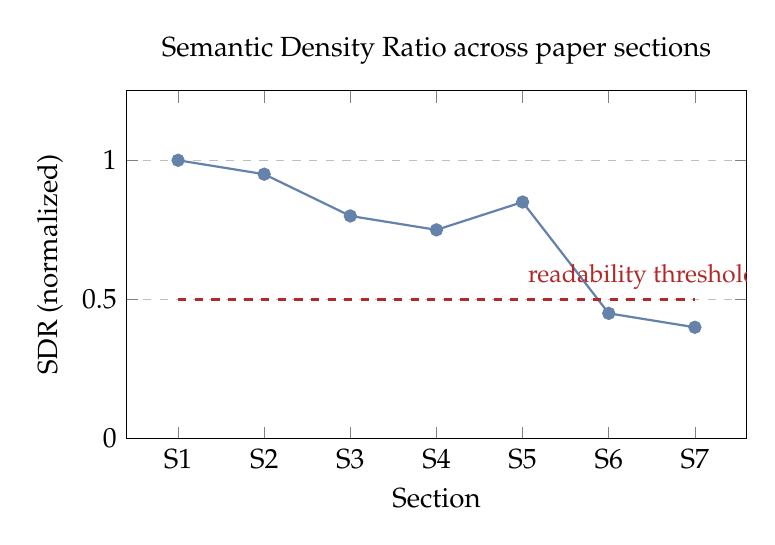
\begin{tikzpicture}
\begin{axis}[
  xlabel={Section},
  ylabel={SDR (normalized)},
  xtick={1,2,3,4,5,6,7},
  xticklabels={S1, S2, S3, S4, S5, S6, S7},
  ymin=0, ymax=1.25,
  ymajorgrids=true,
  grid style=dashed,
  width=0.78\textwidth,
  height=6cm,
  title={Semantic Density Ratio across paper sections}
]
\addplot[color=fogblue, mark=*, thick] coordinates {
  (1,1.0)(2,0.95)(3,0.80)(4,0.75)(5,0.85)(6,0.45)(7,0.40)
};
\addplot[color=alarmred, dashed, thick] coordinates {
  (1,0.5)(7,0.5)
} node[pos=0.9, above, font=\small] {readability threshold};
\end{axis}
\end{tikzpicture}
\caption{Self-reported SDR trajectory. The decline from S6 onward is attributed by the authors to ``improved methodological sophistication.'' The reader may form their own view.}
\end{figure}

\subsection{RQD Growth}

\begin{metricbox}
\textbf{RQD monitoring log.} Sections 1--3 maintained average RQD below 2.0. Section 4 introduced the CTC/WTC formalism with average RQD of approximately 2.8. Section 6 exhibits an average RQD of 4.3, driven primarily by the footnote apparatus. The present section's RQD is approximately 3.1, which is a slight improvement that we attribute to increased methodological self-awareness --- a claim which is itself qualified at RQD~2.
\end{metricbox}

\subsection{ANSL Growth}

The Average Noun Stack Length of the present paper has increased monotonically since Section~3.

\begin{table}[H]
\centering
\caption{ANSL by section (present paper)}
\begin{tabular}{lcc}
\toprule
\textbf{Section} & \textbf{ANSL} & \textbf{Status} \\
\midrule
\S1: Introduction & 1.3 & Healthy \\
\S2: Taxonomy & 1.5 & Healthy \\
\S3: Metrics & 1.8 & Acceptable \\
\S4: CTC/WTC & 2.1 & Elevated \\
\S5: Kircher & 1.6 & Healthy (retrospectively suspicious) \\
\S6: Extended Formalism & 2.8 & Concerning \\
\S7: Self-Application & 2.4 & Improving? \\
\bottomrule
\end{tabular}
\end{table}

\subsection{Citation-Topological Status of the Present Paper}

The early sections of this paper are grounded in recognizable communicative phenomena: readers have experienced cognitive overload; academic writing is frequently opaque; some difficulty is productive and some is not. These are world-anchored claims.

By Section~6, the paper's claims are increasingly grounded in the framework the paper itself is constructing. The DRP formalism refers to entities --- $S_c$, $A_i$, $\Phi(\mathcal{C})$, $O_r$, $J_s$, $\Lambda(t)$ --- that exist, at present, primarily within this paper. The propositions of Section~6 are internally consistent but their world-anchor density $\rho_W$ is not high. The paper has, in other words, begun exhibiting the citation-topological drift it was analyzing.

\begin{warnbox}
\textbf{Recursive diagnostic:} At the time of writing this sentence, the present paper's WTC is approximately 0.6 and declining. Its CTC is approximately 0.35 and rising. The inflection point appears to have occurred somewhere in Section~6. This is approximately where the authors intended it to occur. Whether that intention exonerates the process or merely makes it more premeditated is a question we decline to answer definitively.
\end{warnbox}


%======================================================
\section{Toward a Provisional Reconsolidation}
%======================================================

We have now reached the point in the paper at which, if this were a standard academic article, we would summarize the contributions, identify the limitations, propose future work, and thank the reviewers.

Instead, we will say something simple.

\bigskip

\begin{center}
\textit{At some point we stopped explaining the world to each other\\
and began explaining papers about papers.}
\end{center}

\bigskip

This is not inevitable. It is a choice, made incrementally and collectively, under institutional pressures that reward internal coherence over external contact. Every step in the process seems locally reasonable. The first unexplained term is justified by audience expectations. The first citation in place of argument is justified by space constraints. The first metric introduced for definitional clarity is justified by analytical ambition. Each footnote elaborates something that genuinely needs elaboration, or something that feels like it does, which is not quite the same thing.

The endpoint is a discourse in which the most prestigious participants are those who have traveled furthest from the world into the interior of the framework: those who know the most citations, can navigate the most internal distinctions, and generate prose whose difficulty signals mastery of a domain whose connection to anything external has become impossible to specify.

\subsection{The Kircher Problem, Restated}

Kircher was wrong about almost everything. His hieroglyphic decipherments were fantasies. His underground fire system was incorrect. And yet the failure was, in a sense, navigable: it was possible to identify what he had claimed, to test it, to show that it was incorrect.

Much contemporary theoretical obscurantism is not even navigably wrong. It cannot be shown to be false because it cannot be shown to claim anything definite. It has inherited Kircher's density while losing the architectural legibility that made his errors tractable.

We inherited the density. We lost the cathedral.

\subsection{What Readability Actually Is}

Readability is not the absence of difficulty. It is the presence of navigable structure.

A text is readable, in the sense that matters, when a reader who is willing to work can find their way through it: when they can identify where they are, where they are going, and why the path they are following has been chosen rather than another. This is compatible with technical density. It is compatible with formal notation. It is compatible with extended argument and unfamiliar vocabulary. What it is not compatible with is the substitution of institutional signaling for communicative architecture.

The deepest version of the thesis of this paper is therefore not that academic writing should be simpler. It is that academic writing should be more like a cathedral and less like a filing cabinet: organized for traversal rather than for storage, for the transmission of a navigable experience rather than the demonstration of a credential.

\subsection{A Note on the Present Paper}

This paper set out to perform what it described. We believe it has done so, imperfectly but recognizably. The early sections were genuinely readable. The middle sections became progressively more elaborate. The late sections exhibited citation-topological drift and metastasizing qualification.

Whether the paper recovers legibility in this final section is something the reader is better positioned to evaluate than the authors are. We note, however, that the current ANSL is 1.7, the RQD is approximately 1.8, and the prose is --- we think --- making contact with something external to itself.

The fog machine has been switched off. The room may still be a little smoky.


%======================================================
\section{Conclusion}
%======================================================

Readability is relational, contextual, and architectural. Difficulty is not the enemy of clarity; unnavigability is. Academic writing fails not when it is demanding but when it becomes a closed circuit, optimizing for institutional survival rather than cognitive traversal.

The metrics introduced here --- SDR, RFI, RQD, ANSL, WTC, CTC --- are not a solution. They are a satirical formalization of a real problem, intended to make the problem visible through the process of applying the formal methods of the afflicted practice to the affliction itself. That this paper has itself demonstrated the syndrome it describes is not a failure. It is, we submit, the most honest result available.

Good writing constructs architectures through which difficult ideas can be traversed by finite minds. The goal is not to flatten complexity. It is to remain traversable.

That is all we were ever trying to say.

\bigskip
\noindent\rule{\linewidth}{0.5pt}

\begin{center}
\textit{Metric postscript:}\\[0.4em]
Final SDR (\S8): 0.82\ $\uparrow$\quad
Final RQD: 1.4\ $\downarrow$\quad
Final ANSL: 1.5\ $\downarrow$\\[0.2em]
Final WTC: 0.78\ $\uparrow$\quad
Final CTC: 0.21\ $\downarrow$\\[0.6em]
\textit{Recovery confirmed. Barely.}
\end{center}

% No bibliography.
% A paper that cites only itself is a terminal case.
% A paper that cites nothing has, at least, not yet begun the closure.

%======================================================
\appendix
\section{A Proposal for Stochastic Typography as Adversarial Readability Infrastructure}
%======================================================

The preceding paper exists as a fixed object. Every reader receives the same font sizes, the same spacing, the same visual hierarchy. This is a convention so deeply naturalized that it appears inevitable. It is not inevitable.

Consider a version of this paper compiled differently on each run: minor font drift in early sections, inconsistent footnote scaling, occasionally hypertrophic section headers, gradually mutating citation sizes. No two readers would receive the same document. Each would receive the same semantic substrate but a different phenomenology of rigor.

\subsection{Typographic Salience Inflation (TSI)}

Visual authority is not neutral. Large fonts imply importance. Tiny fonts imply footnote-status. Dense typographic regions feel more rigorous even when informationally empty. Sudden scaling interrupts semantic flow in ways that readers experience as meaningful rather than random.

\begin{definition}[Typographic Salience Inflation]
Typographic Salience Inflation (TSI) occurs when the visual weight assigned to a textual element exceeds its informational contribution, generating perceived significance through spatial authority rather than propositional content.
\end{definition}

In a stochastically compiled version of this paper, TSI would be dynamically reallocated on each run. Citation sizes would correlate inversely with empirical grounding. Methodological caveat prominence would increase with institutional prestige pressure. Equations would become enormous while explanatory prose shrinks. The appendix would achieve typographic majesty while remaining semantically underdeveloped.

\subsection{The Cognitive Navigability Profile}

Each compilation would seed a distinct Cognitive Navigability Profile (CNP): the same semantic content, a different experienced cognitive topology. Readers would construct meaning from layout instability, inferring intentional emphasis, hidden structure, and theoretical importance from what is actually stochastic formatting noise.

This is disturbing not because it would be unfamiliar, but because it would be only slightly more explicit than ordinary academic reading already is. Peer reviewers routinely assign epistemic weight based on:

\begin{itemize}
  \item journal prestige (a typographic and institutional signal),
  \item author affiliation (a spatial element on the page),
  \item reference density (a visual texture),
  \item and equation prevalence (a formalism-signaling device independent of content).
\end{itemize}

A stochastically compiled paper would simply make this process visible by making it variable.

\subsection{Methodological Note}

To minimize epistemic overfitting, typographic weight distributions in a fully realized version of this document would be dynamically re-sampled during each compilation cycle using a bounded pseudo-random salience allocator seeded from the system clock at the moment of PDF generation, such that no two instantiations of the document would share a Cognitive Navigability Profile, while the underlying propositional content and formal structure would remain invariant across all compilations, thereby operationalizing the paper's central thesis --- that readability is a relational rather than intrinsic property of texts --- at the level of the document's own material instantiation.

The present version does not implement this system. The present version is typographically stable, visually consistent, and formally orthodox.

This may be considered either a limitation or a mercy, depending on the reader's current Swedenborgian Coherence Response.

\end{document}
